% options:
% thesis=B bachelor's thesis
% thesis=M master's thesis
% czech thesis in Czech language
% slovak thesis in Slovak language
% english thesis in English language
% hidelinks remove colour boxes around hyperlinks

\documentclass[thesis=B,czech]{FITthesis}[2012/06/26]

\usepackage[utf8]{inputenc}

% \usepackage[unicode]{hyperref}
\usepackage{listings}
\usepackage{graphicx} %graphics files inclusion
% \usepackage{amsmath} %advanced maths
% \usepackage{amssymb} %additional math symbols

\usepackage{dirtree} %directory tree visualisation

% % list of acronyms
% \usepackage[acronym,nonumberlist,toc,numberedsection=autolabel]{glossaries}
% \iflanguage{czech}{\renewcommand*{\acronymname}{Seznam pou{\v z}it{\' y}ch zkratek}}{}
% \makeglossaries

\newcommand{\tg}{\mathop{\mathrm{tg}}} %cesky tangens
\newcommand{\cotg}{\mathop{\mathrm{cotg}}} %cesky cotangens

% % % % % % % % % % % % % % % % % % % % % % % % % % % % % % 
% ODTUD DAL VSE ZMENTE
% % % % % % % % % % % % % % % % % % % % % % % % % % % % % % 

\department{Katedra \ldots (softwarového inženýrství)}
\title{ InfoWeb - Nástroj získávání informací z webů }
\authorGN{Jakub} %(křestní) jméno (jména) autora
\authorFN{Tuček} %příjmení autora
\authorWithDegrees{} %jméno autora včetně současných akademických titulů
\supervisor{Ing. Jiří Hunka}
\acknowledgements{Chtěl bych poděkovat za trpělivost vedoucímu, Ing. Jiřímu Hunkovi.}
\abstractCS{V~několika větách shrňte obsah a přínos této práce v~češtině. Po přečtení abstraktu
by se čtenář měl mít čtenář dost informací pro rozhodnutí, zda chce Vaši práci číst.}
\abstractEN{Sem doplňte ekvivalent abstraktu Vaší práce v~angličtině.}
\placeForDeclarationOfAuthenticity{V~Praze}
\declarationOfAuthenticityOption{4} %volba Prohlášení (číslo 1-6)
\keywordsCS{Nahraďte seznamem klíčových slov v češtině oddělených čárkou.}
\keywordsEN{Nahraďte seznamem klíčových slov v angličtině oddělených čárkou.}

\begin{document}

% \newacronym{CVUT}{{\v C}VUT}{{\v C}esk{\' e} vysok{\' e} u{\v c}en{\' i} technick{\' e} v Praze}
% \newacronym{FIT}{FIT}{Fakulta informa{\v c}n{\' i}ch technologi{\' i}}

\begin{introduction}
V předmětech BI-SP1 a BI-SP2 v prostředí FIT ČVUT byl realizován týmový projekt umožňující získávání informací z webů s primárním zaměřením na potřeby obchodů. Projekt řešil problém automatizace získávání dat z webů, jelikož stávající služby neposkytují veřejné rozhraní
nebo mají velkou chybovost dat.
\par
Práce pojednává o požadavcích internetových obchodů, které jsou především tvořeny nutností držet krok s trhem a sledovat vývoj cen
prodávaných produktů u konkurence.
\par
Cílem této práce je popsat požadavky internetových obchodů, stávající stav získávání informací z webů a možná řešení problematiky. Dále na základě těchto poznatků zhodnotit vytvořené řešení a včetně korektnosti zvolených postupů navrhnout vylepšení. Ty implementovat, řádně vylepšení
otestovat a zhodnotit výsledný stav projektu.


\newpage

\end{introduction}


\chapter{Popis problematiky získávání informací z webů}

V této kapitole se budu nejprve zabývat samotnou problematikou získávání informací 
z webů s důrazem na internetové obchody.
Jelikož je tato problematika již řešena existujícími službami, existující služby zhodnotím.

\section{Problematika}
Získávání informací z webů je efektivní možnost jak získat databázi informací, které se na internetu vyskytují.
Tato činnost však stojí na problematice data získávat a uchovávat v potřebné struktuře, jelikož 
jinak z dat nejsme schopni vyčíst potřebné informace.
Vzhledem k specificitě dat, které jsou v kontextu činnosti zajímavá a dále kvůli unikátnosti webových stránek
není možné jednoznačně určit jednotný a zcela automatizovaný postup, jak data získat v požadovaném formátu.

\section{Výběr dat}
Nejčastější řešení je kombinace automatizace a prvku lidské inteligence.
To je obvykle dosaženo roboty, kteří data stahují a lidské práce určující jaké informace nás ve stažených datech zajímají.
\par
Získávání informací ze stažených stránek lze poté zjednodušit na problematiku určení elementů v HTML, které jsou pro 
nás zajímavé.
Lokaci elementu v HTML se kterým je potřeba pracovat lze poté jednoznačně určit například pomocí těchto dvou možností:
\begin{enumerate}
\item XPath
\item CSS Selector
\end{enumerate}

\section{XML Path Language}
XML Path Language\cite{XPath} nazývaný zkráceně XPath je jazyk, který slouží k výběru elementu v dokumentu ve formátu XML\cite{XML}.
\par
XML chápeme jako jazyk popisující strukturu dat, které jsou strojově i lidsky čitelné.
HTML lze chápat jako strukturu podobnou XML, ačkoliv se přímo o XML dokument nejedná \cite{HTML}. 
HTML popisuje obsah dat pro prezentaci ve webovém prohlížeči pomocí předem definované struktury, které prohlížeče rozumí.
Díky této vlastnosti lze použít XPath pro definování cesty k prvku, který uchovává potřebnou informaci na webové stránce.
\par
\section{CSS Selector}
Jazyk CSS je používán pro vizuální popis prezentace webové stránky definované v HTML. K určení prvků se kterými
pracuje používá selektory, které označují tento prvek v HTML Buď pomocí samotného prvku, přiřazené třídy nebo
identifikátoru. Jako selektor může být použit jak samotný název prvku,
tak vlastní definované třídy.\cite{CSS}
\par
Pomocí řetězení těchto selektorů je poté možné jednoznačně získat element v HTML dokumentu.

\newpage

\section{Současný stav řešení potřeb internetových obchodů}
I v kontextu malého trhu jako Česká republika se lze bavit o velké konkurenci na poli 
maloobchodů prodávající své zboží na internetu.
Internetové obchody potřebují monitorovat konkurenci a trh. Vzhledem k jejich zaměření je tedy nejvíce zajímají 
obchody prodávající stejné zboží. Potřebné informace o prodávaných produktů konkurencí 
se skládají z následujících atributů:

\begin{enumerate}
\item Název
\item Model
\item EAN
\item Cena
\item Inzerovaný název
\item Dostupnost
\end{enumerate}

S těmito daty je poté možné dále pracovat, například při analýze konkurence schopnosti na trhu. \cite{hunka}

\subsection{Srovnávače cen}

Data lze získat pomocí srovnávačů cen jako \textit{zbozi.cz}\cite{heureka} 
nebo \textit{heureka.cz}\cite{zbozi}. Problém u těchto služeb spočívá v určení pro koncové zákazníky, kterým umožňuje
pro nalezení nejlepší ceny na trhu pro hledaný produkt. S tím souvisí to, že největší srovnávače cen neposkytují veřejně 
svá data nebo rozhraní přes která by je bylo možné jednoduše získat.
\par
V rámci výzkumu pro bakalářskou práce jsem měl možnost nahlédnout do dat, které \textit{heuréka} poskytuje některým obchodům. \cite{hunka}

Data obsahují následující informace:
\begin{itemize}
\item Informace o produktu - Segment, Kategorie, Jméno, ID, Výrobce, EAN, Item ID
\item Url na vlastním obchodu
\item Url na heuréce
\item Počet konkurence a popularita na trhu
\item Vlastní cena a pozice dle ní
\item Deset nejvyšších a nejnižších cen
\end{itemize}

První zásadní nedostatek zprávy z jmenovaného srovnávače, se ukázal být logistický a to, že obchod musí být označen \uv{Ověřeno zákazníky},
aby měl k datům přístup. Další nedostatek jsou data neobsahují konkrétní označení konkurenčních obchodů.\cite{heureka-report}
Vzhledem k povaze struktury a splatnosti generovaných dat je také nemožné ceny sledovat v časovém období.
Ostatní srovnávače mají údajně výstup velmi podobný nebo jako bylo výše řečeno, data neposkytují. Díky tomu se ukázali
srovnávače jako nedostatečný zdroj dat.\cite{hunka}


\subsection{Existující služby}

Problematiku sledování trhu s důrazem na firemní klientelu, řeší aktuálně několik existujících služeb.
\par
Služby mají v zásadě velmi podobnou povahu poskytovaných možností. Rámcově se jedná o porovnávání cen včetně historie na různých internetových
obchodem či na srovnávačích. Uživatel si zadá okruh či seznam produktů, buďto formou manuální či vstupem ze souboru, případně 
přímých napojením na e-shop. Následně je možné konkrétní data zobrazit v grafech označující vývoj cen, trendů či náhlých změn.
Dále umožňují externí výstup do souboru v dostupných formátech.
\par
Největší rozdíl služeb je zda jsou data získávána přímo z obchodů nebo ze srovnávačích. Další odlišností je 
možnost zda služba dokáže sledovat i zahraniční trh.
\par
Cena služeb se nejvíce odvíjí od počtu sledovaných produktů a četnosti aktualizací. Proto se měsíční platby mohou 
pohybovat od stovek korun po desítek tisíc korun.

\section{Popis konkrétních existujících služeb}

\subsection{Price checking\cite{priceChecking}} 


\textbf{Hlavní funkce}
\begin{itemize}
\item porovnává a vyhledává ceny zadaných výrobků v reálném čase
\item sleduje dostupnost produktů
\item automatické stahování dat v intervalech
\item statistické pohledy, nahlížení do historie
\item generování grafů
\item cenotvorba
\end{itemize}

\textbf{Vstup}
\begin{itemize}
\item souhrn produktů určený pro sledování
\item libovolný formát, například xsl nebo xml
\item možný manuální vstup
\end{itemize}

\textbf{Výstup}
\begin{itemize}
\item libovolný formát, například xsl nebo xml
\item webové rozhraní
\end{itemize}

\textbf{Prostředí}
\begin{itemize}
\item webové rozhraní
\end{itemize}

\textbf{Data}
\begin{itemize}
\item přes 250 výrobců, 300 obchodů a 1 200 000 výrobků
\item český, slovenský, polský, slovinský, německý a maďarský trh
\item aktualizace denně, maximálně 144 krát za den
\item počet sledovaných obchodů je fixní, lze však přidat na požádání
\item převážně elektronika, bílé zboží, pneumatiky a hračky
\end{itemize}

\textbf{Cena}
\begin{itemize}
\item 6000 - 85 000 Kč (bez dph) za licenci měsíčně
\item minimální doba smlouvy 12 měsíců
\end{itemize}

\begin{figure}[h]\centering
 	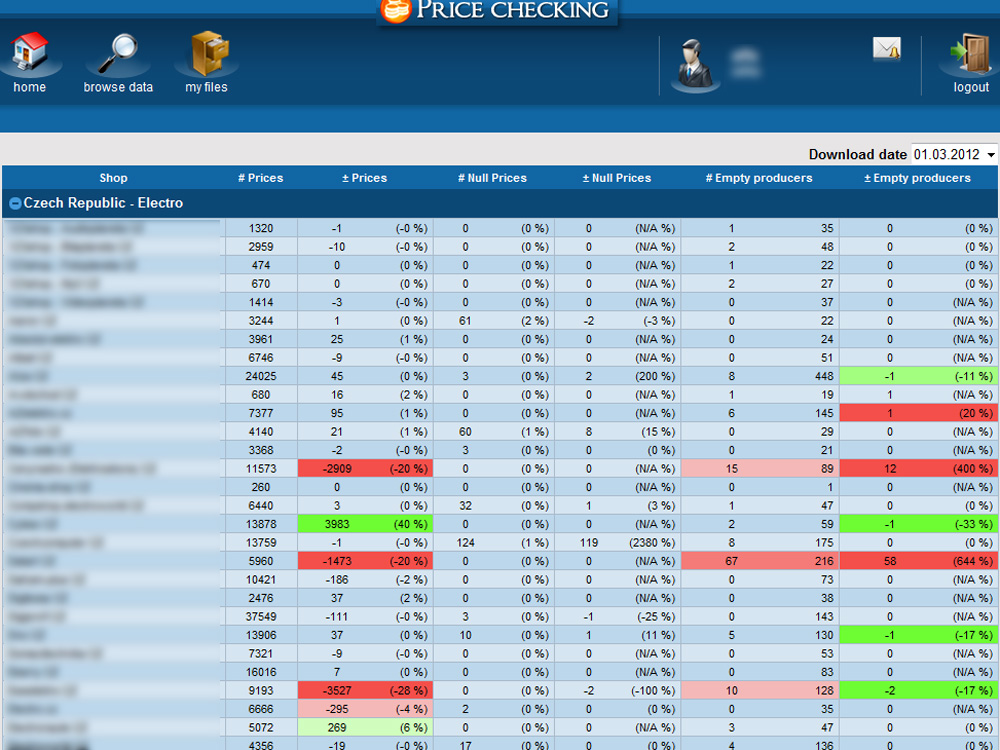
\includegraphics[width=0.9\textwidth]{resources/priceChecking}
	\caption[Price checking]{Ukázka služby price checking}\label{fig:priceChecking}
\end{figure}

\newpage

\subsection{Pricing intelligence\cite{pricingIntelligence}} 

\textbf{Hlavní funkce}
\begin{itemize}
\item monitorování a srovnávání cen konkurence, vývoj cen a trendů v čase
\item přehledné výpisy výsledků
\item u většiny cenových nabídek nutno definovat počet konkurentů
\item upozornění na změny cen v čase
\end{itemize}

\textbf{Výstup}
\begin{itemize}
\item formát xsl nebo pdf
\end{itemize}

\textbf{Prostředí}
\begin{itemize}
\item webové rozhraní
\end{itemize}

\textbf{Data}
\begin{itemize}
\item nespecifikované data a zaměřený trh
\end{itemize}

\textbf{Cena}
\begin{itemize}
\item 599 až 4999 Kč měsíčně
\item minimálně tři měsíce
\item neomezené sledování produktů a konkurentů je možné pouze s nejvyšším tarifem a po individuální ceně
\end{itemize}


\subsection{Sledování trhu\cite{sledovaniTrhu}} 
\textbf{Hlavní funkce}
\begin{itemize}
\item sledování cen, pozic, dostupnosti a hodnocení na porovnávačích zboží i jednotlivých obchodech
\item uchování historie
\item možné napojení přímo na vlastní internetový obchod
\item notifikace změn
\item možnost více účtů s oddělenými přístupy
\item cenotvorba
\item detekce cenových spirál (kdo první zlevnil a následující dopady)
\end{itemize}

\textbf{Vstup}
\begin{itemize}
\item xml, xsl nebo manuálně
\end{itemize}

\textbf{Výstup}
\begin{itemize}
\item xsl nebo webový
\end{itemize}

\textbf{Prostředí}
\begin{itemize}
\item webové rozhraní
\end{itemize}

\textbf{Data}
\begin{itemize}
\item srovnávače cen: heureka.cz, zbozi.cz, najnakup.sk, pricemania.sk, ceneo.pl, nokaut.pl, argep.hu, preisroboter.de
\item přímé sledování na obchodu
\item z toho plyne záběr na český, slovenský, německý a maďarský trh
\item aktualizace až několikrát denně
\end{itemize}

\textbf{Cena}
\begin{itemize}
\item platba za každé vyhledání
\item individuální cena
\end{itemize}

\subsection{Pricebot \cite{priceBot}}

Web je datován roku 2015, avšak popis funkcí není dokončený. Obsahuje výplňový text, proto je popis funkcí nekompletní.

\textbf{Hlavní funkce}
\begin{itemize}
\item denní monitoring cen na heureka.cz
\item možnost sledovat produkty konkurence
\item poskytuje pravidelný výsledek nalezených cen a vizualizaci změn
\item notifikace o změnách
\item notifikace o konkurentech prodávajících za nižší cenu
\item maximum lze sledovat 600 produktů 
\item maximum sledovaných konkurentů je 70
\end{itemize}

\textbf{Vstup}
\begin{itemize}
\item produkty ke sledování
\end{itemize}

\textbf{Výstup}
\begin{itemize}
\item pdf na email
\end{itemize}

\textbf{Prostředí}
\begin{itemize}
\item webové rozhraní
\end{itemize}

\textbf{Data}
\begin{itemize}
\item srovnávač cen Heureka.cz
\end{itemize}

\textbf{Cena}
\begin{itemize}
\item dle počtů produktů
\item od 299 do 1299 Kč
\end{itemize}

\newpage

\subsection{Zahraniční nástroje}
Tyto nástroje jsou obecněji zaměřené a obvykle požadují od uživatele techničtější zaměření, 
jelikož je nutné přesně specifikovat kde, co a jak chce sledovat. Vzhledem k tomuto omezení
nejsou přímo pro provozovatele e-shopů vhodné kvůli nedostatečným technickým kapacitám a 
pro tuto práci důležité.
\par
Příklad zahraničních nástrojů:

\begin{enumerate}
\item Screen scraper \cite{ScreenScraper}

  \begin{itemize}
    \item Webová služba
    \item procházení web skrz odkazy
    \item potvrzování formulářů
    \item využití interního vyhledávání
    \item export do širokého množství formátu souborů
    \item cena: \$549 - \$2,799 za měsíc
  \end{itemize}
  
\item Web extractor \cite{WebExtractor}

  \begin{itemize}
    \item Windows Aplikace
    \item procházení zadaných stránek
    \item hledání stránek pomocí klíčových slov
    \item export do csv formátu
    \item cena: \$99 - \$199 jednorázově
  \end{itemize}


\end{enumerate}

\newpage

\chapter{Analýza týmového projektu}
V kapitole analýza týmového se budu věnovat řešení vytvořeného v rámci školní výuky na ČVUT FIT v akademickém roce 2015/16.
Nejprve popíšu cíl, který měl projekt za úkol řešit, jaké byly použité postupy při vývoji a mou roli v tomto projektu.

\section{Cíl týmového projektu}

V předmětech BI-SP1 a BI-SP2 byl realizován týmový projekt, v souladu s osnovami těchto předmětů byl nejdříve v BI-SP1 vytvořen návrh
systému a v BI-SP2 implementován.
\par
Cíl který projekt řešil, byla maximální možná míra automatizace získávání informací o produktech prodávaných konkurencí. Důraz je především kladem na optimalizaci počtu nutných lidských úkonů administrátora u kterého se předpokládá minimální technické vzdělání.
Jediná nutná problematika, co tak musí administrátor ovládat je parsování HTML stránek.
\par
Návrh popisuje rozdělení aplikace na část poskytující veškeré webový rozhraní a na část zpracovávající všechny interní procesy.
Vzhledem k požadavkům na škálovatelnost aplikace, druhá část se skládá z více samostatných menších služeb - modulů komunikující
spolu pomocí front. Díky tomu, že každý modul zajišťuje určitou funkcionalitu umožňující vytvářet více jeho instancí, je možné
procesy zpracovávat paralelně. 
Uživatelská a interní část spolu sdílejí data pomocí relační databáze\cite{DB}.

\section{Webové rozhraní}
Webové rozhraní lze rozdělit na dvě části. Uživatelskou část, obsahující množinu podstránek určených pouze pro konečné uživatele
služby a část pro administrátory, sloužící k monitorování kampaní a řešení chyb. Webové rozhraní používá databázi, která pak 
obsahuje všechny uložené a získané data.
\par
Uživatelská část umožňuje vytvořit kampaň. Kampaň je proces trvající určitý časový úsek, který sleduje vložené produkty na konkurenčních
obchodech.
V rámci těchto běžících kampaních má poté uživatel možnost uživatel vidět vizualizaci získaných dat, případně je umožněn export dat do formátu
csv nebo xlsx. Získaná data obsahují, kde se sledované produkty nacházejí a za jakou cenu se prodávají.
\par
Druhá část je určena pouze pro administrátory a slouží k monitorování kampaní uživatelů a řešení chyb, které systém není schopný 
automaticky vyřešit. Chyby jsou typicky problémy s parsováním webových stránek, párování produktu ke stránce nebo potvrzení zda jsou získaná data validní.
\section{Interní část}
Interní část je rozdělena do samostatných modulů, které spolu komunikují pomocí front. Moduly je poté možné spustit jako služby ve více 
instancích. Vzhledem k možnostem front, je pak možné práci distribuovat na více serverech, aniž by byla ohrožena bezpečnost
databáze, jelikož k té je možný přístup pouze lokální. Moduly jsou detailně popsány v následujících podsekcích.
\subsection{Manager}
Manager je hlavní modul, který má jako jediná interní část možnost připojení do databáze a jeho běžící instance může existovat pouze jednou.
Manager má za úkol plánování práce pro ostatní části systému a zpracování vstupů a výstupů z front.
\subsection{Finder}
Finder je modul, který má za úkol získávat URL adresy internetových obchodů a na nich vyhledávat URL adresy vedoucí na požadované detaily produktů.
Detailem produktu je myšlena webová stránka, kde jsou obsažený podrobné informace o prodávaném produktu. Obchody samotné jsou
získávány pomocí vyhledávání na internetových srovnávačích. K vyhledání je použit název produktu. 
\subsection{DataProvider}
DataProvider je modul, který zpracovává adresy vedoucí na detaily produktu. Zde existují čtyři hlavní větve možností zpracování požadavků.
Po stažení stránky, se z ní pokusí získat požadované
hodnoty. V případě neúspěchu odešle příslušnou chybu, v opačném případě zanalyzuje korektnost získaných cen vůči historickým datům pokud
existují. Výsledek je poté odeslán k zpracování  \uv{Managerem}.

\begin{figure}\centering
 	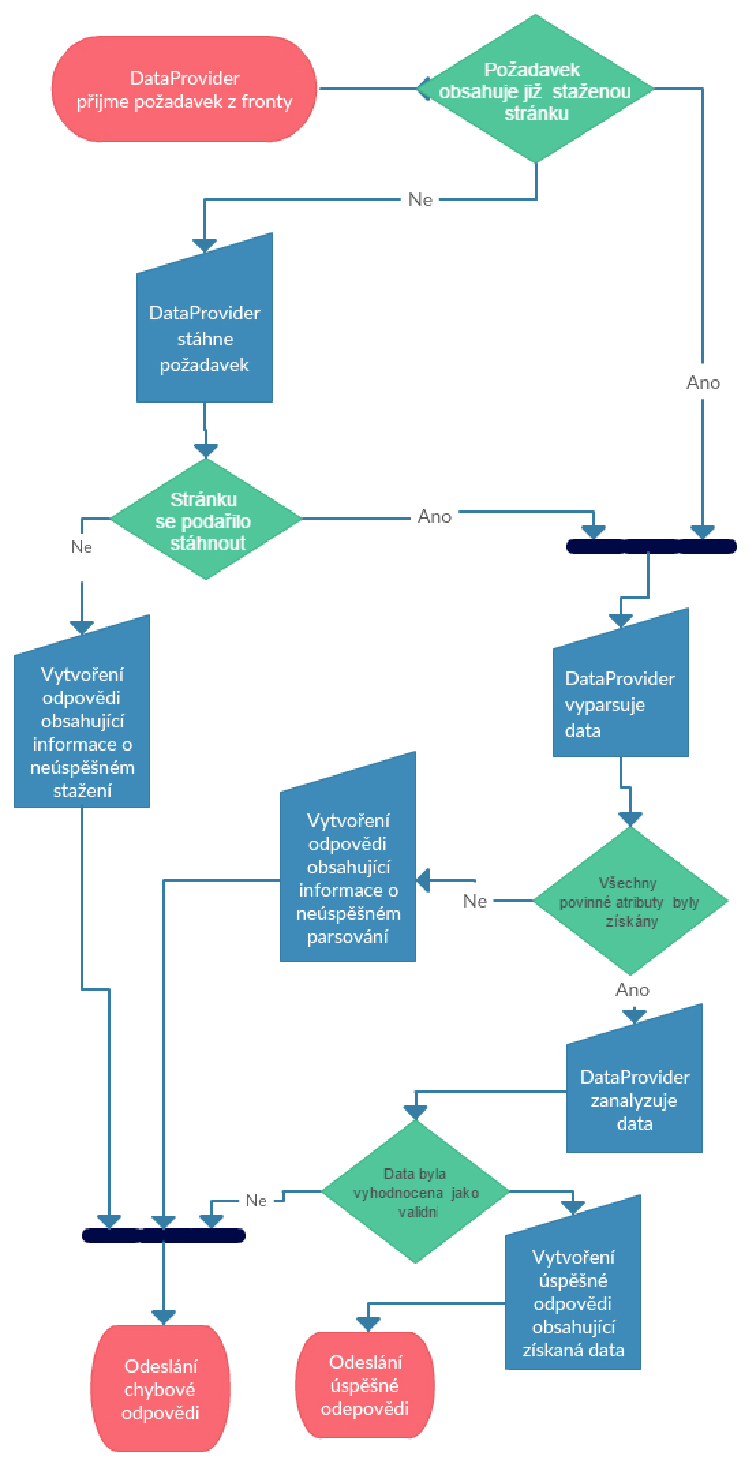
\includegraphics[width=0.8\textwidth]{resources/DataProvider-activity}
	\caption[DataProvider diagram]{Diagram zobrazující aktivity v DataProvider modulu}\label{fig:dp}
\end{figure}

\chapter{Vývoj a implementace týmového projektu}
V této kapitole se věnuji průběhu vývoje týmového projektu a vytvořenému řešení. Poslední část rozebírá mou roli v tomto
projektu, jelikož jsem věděl, že budu téma dále rozvíjet v rámci bakalářské práce. 
Z tohoto důvodu jsem se projektu věnoval nad rámec předmětu. 

\section{Pojmy}

\subsection{Verzovací systém Git}
Git \cite{GIT} je verzovací systém umožňující sdílení jednotlivých verzí verzovaného projektu.
Umožňuje jednoduchý přehled nad rozpracovanými částmi každého vývojáře. Úložiště systému se nazývá repositář, který obsahuje veškerý kód.
Repositář pak existuje v lokálních verzi a zároveň serverové. Sdílený repozitář pak zajišťuje distributivitu mezí všemi
potřebnými členy. Pro lepší správu pak existují nadstavby nad serverovou částí repozitáře, které umožňují jednoduchou
správu nad kóde a spouštění úkolů v závislosti na definované akce. Zde například spuštění sestavení nebo notifikace
při nové změně.
\par
Základní jednotkou tvoří verze, které jsou postupně vytvářeny vývojáři po vytvoření každé malé funkcionality.
Verze jsou poté uchovávány v jednotlivých větví programu. Vedlejší větve slouží pro samotnou postupnou práci. 
Hlavní větve poté tento kód spojují. Git také zajišťuje základní nástroje pro slučování kódu v případě spojování 
nebo slučovaní vedlejších větví do větví hlavních.

\newpage

\begin{figure}[h]\centering
 	
\includegraphics[width=0.7\textwidth]{resources/branches}
	\caption[Větve v Git repozitáři]{Zobrazení větví v repozitáři, kde \textit{master} je hlavní, \textit{develop} vývojová a \textit{topic}
	představuje větev vedlejší}\label{fig:vetev}
\end{figure}

\subsection{Jednotkové a integrační testy}
Jednotkovými testy se rozumí sada kladných a záporných testů ověřující funkcionalitu pouze jedné třídy. Jednotkové testy
jsou nezávislé na ostatních třídách a testech. \cite{testing} 
Integrační testy pak pokrývají komunikaci více tříd nebo komunikaci s operačním systémem, hardwarem či rozhraním různých systémů. \cite{testing}
\par
Důvod psaní testů je lehčí nalezení chyby a lepší udržovatelnost projektu. V případě neexistujících testů nelze poté ověřit původní
funkcionalitu při modifikaci aplikace, což může způsobit nutnost chyby nalézt a opravit.\cite{testing}

\subsection{Statická analýza kódu}
Statická analýza kódu je analýza softwarového produktu, která běží bez spuštění samotné aplikace. Kontroluje 
pouze samotný kód. Označuje kritické konstrukce vedoucí k chybám nebo nedodržení programátorských konvencí daného
jazyka.
\subsection{Průběžná integrace}
Průběžnou integrací se rozumí sada nástrojů sloužící k urychlení softwarového vývoje. Princip je průběžné sestavení
a spouštění testů aplikace na základě změny ve sdíleném repozitáři. Lze tak rychle odhalit případné chyby před zařazením 
příslušné verze do produkce.\cite{CI}

\subsection{Sdílení dat pomocí front}
Princip sdílení dat pomocí front je na odesílání zpráv, které reprezentují objekty. Fungují na principu, kdy jedna strana objekty
odesílá a druhá přijímá. Příklad takové implementace pak může být například RabbitMQ. \cite{rabbitMQ}

\section{Vývoj}
Vývoj byl rozdělen do 5 iterací, z nichž každá obsahovala 10 sprintů. Před začátkem vývoje byla rozdělena práce do těchto částí, 
s tím, že na konci každé iterace probíhala prezentace vyučujícímu. Každý sprint se skládal z jednotlivých
úkolů, které byly přiřazeny členům týmu. Stav úkolů byl uchováván na systému Redmine\cite{Redmine}, ten umožňuje přehledné řízení projektu
a možnost sledování objevených chyb.
\par
Jako verzovací systém byl zvolen systém Git, se vzdáleným repozitářem uložený na službě \cite{gitlab}. Gitlab poskytuje webové rozhraní pro snadnou správu a spouštění služeb na základě změn. Projekt byl v rámci repozitáře rozdělen na 4 části (větve):
\begin{itemize}
\item Master - hlavní větev uchovávající verze určená k nasazení na produkční server
\item Develop - vývojová větev obsahující aktuální stav vývoje
\item Feature - vedlejší větev vytvořená pro konkrétní úkol přidávající novou funkcionalitu
\item Fix - vedlejší větev určená pro úkoly opravující nalezenou chybu
\end{itemize}
Jelikož přístup k přidání verze do Master a Develop měl pouze vedoucí projektu, musel být pro každou Feature a Fix větve
vytvořen požadavek o zařazení. Po kontrole vedoucím byl požadavek zařazen nebo vrácen k opravě.
\par
Na konci každé iterace byla poslední verze vždy označená ve verzovacím systému a poté prezentována vedoucímu.
Označení bylo zvoleno na základě pořadí iterace. 1. iterace je označena verzí \uv{0.1}.
\par
Pro vývoj se využil princip průběžné integrace. Každá verze byla zkompilována, otestována a zanalyzována na vzdáleném serveru.
Tyto činnosti zajišťovaly systém Jenkins\cite{jenkins} a Gitlab. Jenkins aplikaci zkompiloval, spustil testy a statickou analýzu kódu 
zajištěnou systémem SonarQube\cite{sonar}. Výsledky poté publikoval ve svém webovém rozhraní a zároveň v rozhraní Gitlab.  
\section{Implementace}


\subsection{Webové rozhraní}
Webové rozhraní je implementováno v jazyce PHP verze 7. Základem aplikace je aplikační rámec Nette\cite{nette}. Nette
obsahuje nástroje pro automatickou správu závislostí, komunikaci s databází, vytváření bezpečných formulářů, zabezpečení
aplikace, šablonovací systém a rozhraní pro tvorbu jednotkových testů. Dále automaticky umožňuje lehké dodržení MVC architektury, která odděluje
prezenční a logickou vrstvu. Zkratka MVC značí Model-View-Controller. V případě projektu je view šablona definující vzhled webové stránky,
controller třídy obsluhují šablony. Modelovou vrstvu poté zajišťují servisní třídy, vykonávající logické části aplikace jako 
například přístup do databáze nebo zpracování formuláře.

\begin{figure}[h]\centering
 	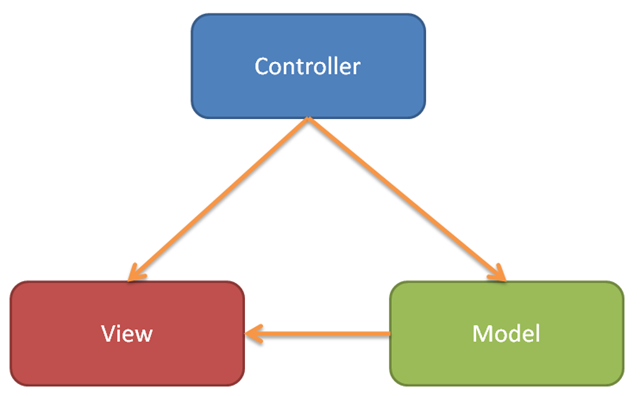
\includegraphics[width=0.7\textwidth]{resources/mvc}
	\caption[MVC]{Vizualizace návrhu MVC (Model-View-Controller}\label{fig:mvc}
\end{figure}
\par
Snadnou správu závislostí umožňuje balíčkovací systém Composer\cite{composer}. 
Na základě souboru definující potřebné knihovny a jejich verze, jsou staženy z centrálního repositáře. To zajišťuje jednotné verze knihovna
a eliminace nutnosti knihovny manuálně stahovat či přímo přidávat do verzovacího systému.
\subsection{Interní část}
Interní část je implementována v jazyce Java verze 8. Kompilaci, spouštění testů a správu závislostí zajišťuje Gradle\cite{gradle}.
Gradle je nástroj sloužící k automatickému sestavení aplikace. Umožňuje správu závislostí, kde je standardně nastavený jako zdroj
centrální maven repositář. \cite{mavenRepo}. Na něm jsou uložené poté všechny knihovny, která jsou v rámci toho projektu použity.
\par
V rámci sestavení lze pustit testy, včetně přídavných doplňků. Projekt používá
doplněk Cobertura\cite{cobertura}, který na základě spuštěné testovací sady vytváří zprávu obsahující pokrytí větví programu.
Díky tomu lze jednoduše zjistit jaké větve aplikace nejsou otestované.
\par
Aplikace je rozdělena do nezávislých modulů běžící jako služby. Jednotlivé moduly spolu komunikují
pomocí posílání zpráv definovaných front. Komunikaci zajišťuje systém RabbitMQ Server implementovaný v jazyce Erlang. Zprávy jsou serializovatelné objekty, jejichž definice je sdílena napříč všemi moduly.
\par
Serializace představuje proces, kdy je objekt serializovaný do posloupnosti bitů, které jsou poslány jako zpráva. 
Vzhledem k sdílené podobě objektu na obou stranách, zprávu lze jednoznačně deserializovat zpět do původní Java objektu se kterým
je poté možné dále pracovat.\cite{serialization}

\par
Použité knihovny:
\begin{itemize}
\item Google Guice - automatická správa závislostí \cite{guice}
\item Hibernate - objektově relační zobrazení databázových entit a práce s nimi \cite{hibernate}
\item Apache Commons - pomocné knihovny pro práci s řetězcemi a soubory \cite{commons}
\item RabbitMQ - zajišťuje komunikaci s frontami \cite{rabbitMQ}
\end{itemize}

\section{Má role}
V druhé části týmového projektu, tedy implementace jsem byl vedoucí týmu. Jelikož jsem se již znal své téma bakalářské práce, 
věnoval jsem se projektu nad rámec předmětu
\par
Především na začátku projektu jsem věnoval čas vytvoření celého ekosystému, tvořen z přidružených služeb použitých při vývoji.
Zde se jedná především o projení následujících služeb s GitLabem:

\begin{itemize}
\item Redmine - možnost prokliku na úkol na základě čísla ve zprávě verzované jednotky (commit message)
\item Jenkins - spouštění sestavení aplikace na základě nové verze, oddělené dle jednotlivých větví (hlavní, vývojová, vedlejší) a
				informace o výsledku
\item SonarQube - zobrazování interaktivního výsledku statické analýzy přímo v rozhraní GitLab
\end{itemize}

Samotný SonarQube bylo nejprve potřeba nastavit, aby se spouštěl při sestavení aplikace a výsledek se poté zobrazil v rozhraní
GitLabu. V rámci sestavení aplikace jsem ještě nastavil spouštění nástroje Cobertura.
Doplňky v Jenkins poté umožňovaly zobrazení přehledných výsledků, jak je kód pokryt testy. Přesné pokrytí testy mi poté umožňovali 
jednoduše kontrolovat, zda jsou správně napsané všechny testy.

\chapter{Zhodnocení týmového projektu}
Pro nutnost návaznosti na kapitolu o vylepšeních je nejprve nutné uvést v jakém kontextu jsou vylepšení navrhovány. K tomu je třeba
popsat výsledný stav projektu a jeho funkcionalitu. 

\section{Pojmy}

\subsection{JSON}
JSON označuje specifikaci formátu pro výměnu dat\cite{JSON}. Jedná se o formát, který je čitelný jak pro lidské oko tak pro stroj\cite{JSON} a jeho zpracování je implementováno pro velké množství programovacích jazyků\cite{JSON-impl}. Základní stavební jednotkou
tvoří kolekce párů klíč a hodnotu spolu se seřazeným polem hodnot.

\subsection{Web API}
Rozhraní, které na definovaný HTTP dotaz vrací data. Ty jsou standardně vracena ve formátech JSON nebo XML.

\section{Stav}
Ačkoliv stav projektu odpovídal nárokům na úspěšné odevzdání nebyla dosažena implementace všech procesů, aby byla umožněno reálné
použití systému.
\par
Odevzdávaný stav obsahoval funkční webové rozhraní, které se skládalo ze základní funkcionality pro uživatele a pro administrátory.
Část pro administrátory obsahovala správu uživatelů, možnost parsování stránek, evidenci známých obchodů a produktů či sledování
chyb vzniklých v interní části.
Uživatelská část umožňovala správu a vytvoření kampaně či kampaní. Implementace kampaní pak splňovala návrh z analytické částí,
která byla zmíněna výše.
Na žádost jiného týmu jsme také vytvořili REST rozhraní, poskytující získané ceny pro daný produktu.
\par
Interní část byla schopná pracovat pouze na základě dříve uložených url adres vedoucí detaily produktů. 
Manager dokázal zjistit vybrat produkty, které jsou v aktivní kampani a je třeba je aktualizovat.
Na základě výsledků poté vybral potřeba data odeslal požadavek pomocí pro zpracování do DataProvideru. Ten na základě obdržených dat stránku vyparsoval a zanalyzoval výsledek vůči historickým datům a informacích o produktu. 
\par
Analýza se především skládala z kontrol velkých výkyvů cen a rozdílných identifikátorů produktu.
V případě, že požadavek neobsahoval šablonu pro vyparsování nebo byl výsledek označen jako chybný a byla odeslána chyba
zpět do Manageru. Manager následně výsledek korektně uložil pro zobrazení ve webovém rozhraní, ať už se jednalo o chybu
nebo nalezení ceny.
\par
Byla také obsažena detekce opravených chyb, díky kterému Manager poznal, že může pokračovat v práci hledání cen na daném.

\section{Nedostatky}
Vytvořené řešení obsahovalo spoustu nedostatků, které je třeba v rámci této práce detekovat a ty nejdůležitější se pokusit opravit.
Z důvodu kontextu a odlišnosti od původního návrhu nejprve popíšu systém plánování práce, který je důvodem mnoha chyba.

\subsection{Vytváření požadavků pro ProductProvider}
Následující nedostatky jsou úzce spjaty s tím, jak aplikace plánovala práci. Plánováním práce je myšleno proces ve kterém 
jsou vybrány požadováné adresy detailů a z nich vytvářeny požadavky pro ProductProvider k zpracování. 
\par
Jak bylo řečeno, prvotním kritériem jsou adresy detailů. Ty se mohou vyskytovat v různých stavech. Systém je vybral v 
následujícím pořadí, z kterého následně vybral první 10:

\begin{itemize}
\item Adresy, které jsou v zaplacené kampani
\item Adresy bez produktů
\item Adresy, pro které neexistuje šablona pro parsování
\item Adresy, které mají vyřešenou chybu
\end{itemize}

Z této množiny byly poté odebrány odeslané a ty které mají nevyřešenou chybu. Opakované spuštění v předefinovaném intervalu poté 
zajistilo, že požadavky byly vytvořeny pro všechny požadované adresy.

\subsection{Neefektivní chování modulu Manager a ProductProvider}
První zásadní problém bylo neefektivní chování komunikace modulu Manager s ProductProviderem. V rámci testování jsem zjistil, že v 
případě chyby při parsování stránky není použit uložený HTML dokument.
To pramenilo z výše popsaného návrhu plánování, které nalezlo korektně adresy, ale vytváření samotného objektu představující požadavek,
bylo stejné pro všechny adresy. Vytváření tedy neobsahovalo použití již staženého dokumentu, na jehož základě byla vytvořena 
chyba parsování nebo analyzování. Každý požadavek tedy vyústil v opětovné stažení příslušné stránky.

\subsection{Chyby analyzování}
Poslední fáze procesu v modulu ProductProvider byla navržena jako analyzování získaných dat vůči již dříve uloženým. Implementace analyzátoru 
spouštěla jednotlivé validace, jejíž logika se nacházela v oddělených třídách. 
Analýza kontrolovala zda se shoduje získaný EAN, název a modelové číslo, vůči uloženým identifikátorům. Pokud na jedné ze stran hodnota neexistovala
byly data označená, že jsou pravděpodobně chybná. Dále probíhala kontrola získané ceny s a bez DPH oproti cenám získané na konkrétní stránce dříve.
Kontrola zde porovnala průměr historických hodnot se získanými cenami. V případě, že rozdíl byl větší jak 25\%, byl výsledek označen jako
možná chyba.
\par
V případě, že validační třída objevila nežádoucí data,
vyhodila výjimku ve které byly uložené informace o chybě. Tento způsob řízení programu však způsoboval, že celá validace skončila při první chybě.
\par
Informace byly následné odeslány a manager na jejich základě vytvořil chybu pro administrátora k vyřešení. Administrátor mohl 
chybu označit jako chybnou. Na základě označení bylo poté vytvořeno nastavení, že daná chyba se má na celém obchodě ignorovat. V opačném případě se adresa přestala používat. Problém nastával pokud se na adrese objevilo více chyb. To znamenalo, že každý další požadavek vytvořil další
chybu analyzátoru a administrátor tak všechny vyřešit a při každém požadavku bylo nutné obsah adresy znova stáhnout.

\subsection{Vytváření chyb šablon}
Jako další problém se ukázalo plánování práce založené na kritériu, kdy jsou k vytvoření požadavku vybrány všechny adresy, které neobsahují šablonu.
Myšlenka byla taková, že pro vytvoření samotné šablony, je nutné nejdříve stránky stáhnout, nechat vyhodit chybu parsování
a nálsdně chybu vyřešit.
\par
Systém však odeslal požadavek pro všechny uložené adresy na obchod. To vyústilo ve vytvoření mnoho chyb, 
které musel administrátor všechny postupně vyřešit.
\par
\subsection{Modul Finder}
Modul Finder nebyl zapojený do systému. Existovala pouze hlavní implementace interních procesů, jejíchž funkčnost byla
pouze ověřena jednotkovými testy. Neexistující rozhraní pro práci s frontami a třídy Managera zajišťující vytváření příslušných požadavků
neumožňovaly ověření celkové funkcionality této části. Z tohoto důvodu nebyl systém jako celek použitelný pro jakékoliv reálné použití, jelikož
jediná možnost jak využít funkcionalitu interní částí, bylo vytvořit SQL insert skripty, obsahující adresy detailů produktů
a ty spustit nad databází, kterou systém používal.
\par
Další důsledek byla neexistence procesu párování produktů. Finder byl navržený tak, že po nalezení internetového obchodu
pomocí interního vyhledávání nalezne detaily produktů, u kterých je velká pravděpodobnost, že patří hledanému produktu.
To je však třeba ověřit. Po získání hodnot ze stránky je tak třeba nežádoucí adresy vyloučit a ostatní spárovat s produktem.
\subsection{Plánování práce}
Projekt neosahoval plánování práce vůči požadovanému intervalu, kdy mají být nová data
staženy. Jak bylo řečeno výše, aktuální stav pouze hledal adresy produktů, které se nachází v zaplacené kampani nebo měli vyřešenou chybu.
\subsection{Škálovatelnost}
Původní návrh počítal se škálovatelností aplikace na více serverech, kde je možné vytvořit neomezený počet instancí DataProvider a Finder. Reálný stav
na konci projektu však tuto možnost nevyužíval, ač to bylo možné. Interní část tak běžela jako jedna služba. Po spuštění
byly inicializovány všechny moduly běžící v samostatných vláknech.
\subsection{Obecný návrh a testy}
Implementace samotná, byla velmi nepřehledná. Vykytovaly se prvky značící špatný návrh aplikace.
Zde bych rád zmínil například dlouhé a nepřehledné metody v
\uv{DataProviderServiceImpl:process a AbstractFinderUrlListWorkerImpl:getProductUrl}, kde ačkoliv jejich velikost 
nepřesahovala 60 řádků bylo velmi obtížné zjistit, co mají vykonávat. Problém byly také velké třídy
jako například \uv{DataProviderServiceImpl} zajišťující celý proces v modulu DataProvider, který byl již zmíněn a popsán výše.
\par
Je nutné podotknou, že spoustu špatných konstrukcí byly eliminovány již v průběhu vývoje týmového projektu.
První důvod byla automatická analýza kódu detekující mnoho konstrukcí, které by se neměly v kódu vyskytovat. Automatická analýza
však nebyla schopná najít všechny problémy. Druhý důvod byla moje kontrola při schvalování vytvořeného kódu pro 
zadaný úkol. Z důvodu časové tísně, ale nebyl vždy čas na to vrátit kód k přepsaní a opravení všech chyb. To způsobilo, že
se vědomě dostaly konstrukce, které nebyly považovány za ideální s myšlenkou, že budou přepracovány později, což se ne vždy povedlo.
\par
Další problém návrhu byly procesy v DataProvider modulu řízené pomocí výjimek obsahující 
přídavné informace i v případech, kdy byl takový výsledek očekávaný nebo dokonce chtěný. 
Toto použití je však v rozporu ideou použití výjimek, které mají signalizovat neočekávaný stav, kdy není možné dále pokračovat.\cite{exception}
Pro uchování přídavných informací bylo nutné vytvářet výjimky vlastní, tak aby byl k údajům možný pozdější přístup.
\par
V kritických částek dále chyběly některé důležité testy, jelikož třídy snažící se dělat více věcí najednou by bylo velmi
složité otestovat. Chybějící testy se vykytovaly například u následujících částí: databázová vrstva, vytváření požadavků pro DataProvider,
hlavní servisní třída DataProvideru nebo validace dat analyzátorem. Z tohoto důvodu jakákoliv oprava nebo implementace nových požadavků 
mohla narušit stávající funkcionalitu bez možnosti rychlého ověření. Tím by mohla být jakákoliv změna velmi časově náročná a s velmi nejistým konečným výsledkem.

Systém proto v tomto stavu nebyl vhodný pro následný rozvoj.

\begin{figure}[h]\centering
 	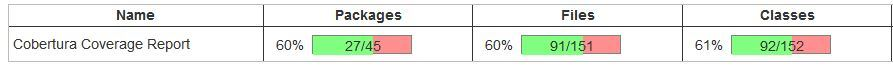
\includegraphics[width=1.0\textwidth]{resources/cobertura-report-old-1}
 	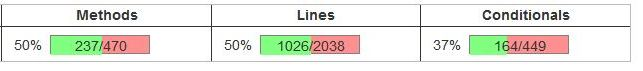
\includegraphics[width=0.7\textwidth]{resources/cobertura-report-old-2}
	\caption[Pokrytí testy vytvořeného řešení]{Pokrytí testy vytvořeného řešení týmového projektu}\label{fig:dp-dia}
\end{figure}


\chapter{Návrhy na vylepšení}
V této kapitole popíšu návrhy možná vylepšení. Tyto návrhy považuji za nejvíce důležité a proto jsou
v rámci této práce i implementované. Samotné implementaci se poté věnuji v následující kapitole. 
Návrhy, které nebyly uskutečněny, jelikož se v době návrhu nezdály tolik důležité nebo byly zjištěny až v průběhu 
vylepšování, budou zmíněny v samostatné kapitole.

\section{Pojmy}

\subsection{Mock}
V objektově orientovaném programování se Mock objekt požívá pro simulování chování konkrétní třídy.\cite{mock}
Při testování je tedy možné docílit testů, které nejsou závislé na ostatních třídách, kromě té která je přímo testována.
Jelikož testovaná třída obvykle vyžaduje závislost na jiných třídách či rozhraní, jsou tyto části pomocí Mocku simulované.
Mimo nadefinování požadovaného chování, lze také na Mock objektu sledovat jaká na něm byly provedené volání, včetně toho
s jakými parametry. Díky tomu je možné testovat i vnitřní chování testované třídy a ne pouze návratovou hodnotu na základě 
obdrženého vstupu.

\subsection{Refaktorování kódu}
Refaktorování v softwarovém vývoji chápeme jako proces restrukturalizace existující kódu, aniž by byla 
pozměněna funkcionalita. Provádí se za účelem dosáhnout průhlednějšího a čitelnějšího kódu, který
se lépe udržuje a rozšiřuje. \cite{refaktoring} Hlavní spouštěcí příčina refaktorování kódu je však existence 
konstrukcí značící špatný návrh aplikace. 

V kontextu této práce jsou důležité především následující konstrukce značící možné problémy: \cite{refaktoring} 
\begin{itemize}
\item Dlouhá metoda
\item Velká třída
\item Dlouhý seznam parametrů
\item Složité struktury podmínek
\end{itemize}

\section{Refaktorování stávajícího řešení}
Vzhledem ke výše popsaným problémům týkající se samotné implementace v interní části, nebylo možné na napsaném kódu stavět
případné opravy nebo celková vylepšení. Z tohoto důvodu by bylo vhodné přepsat téměř celou interní část, tak aby bylo možné
kód lépe udržovat. Zároveň se pokusím z důvodů efektivních, zachovat co nejvíce původních částí. Obzvlášť takové, které jsou ověřeny
že fungují pomocí testů a testovaní. Při přepsání se tedy budu především věnovat nastavení komunikace jednotlivých tříd mezi sebou.
Kvůli tomu bude potřeba změnit jejich komunikační rozhraní, nicméně vnitřní logická funkcionalita by měla ve většina případů zůstat
stejná.
\par
Dále pro větší přehlednost by bylo vhodné přesunou všechny servisní třídy do samostatného balíku a sjednotit je. Jednotlivé funkcionality
budou poté v samostatných balíčcích.


\subsection{Řízení aplikace}
Aplikace, především v modulu ProductProvider, byla řízena pomocí chytání výjimek obsahující informace o chybě. Výjimky by bylo vhodné 
odstranit a návratové hodnoty změnit na objekt obalující celkový výsledek. Tento návrh poté ulehčí běh procesů, kde není žádoucí
skončit při první chybě. Kód bude možné lépe rozdělit a metody následně zkrátit, což výrazně zlepší přehlednost kódu.


\section{Oprava komunikace Manager - ProductProvider}
Vzhledem k problémům zmíněných výše, je třeba komunikaci těchto dvou modulů optimalizovat. Neefektivní chování je
velký problém při zpracování velkého počtu dat, především při nutnosti opakovaného stahování webových stránek. Při analýze kódu se ukázalo, že v aktuálním návrhu aplikace není možné tuto funkcionalitu jednoduše implementovat, aniž by se nejednalo o rychlou opravu, která může způsobit nefunkčnost systému. Rychlá oprava by znamenala, že pro každou vytvářenou adresu je nutné se nejdříve pokusit najít vyřešenou chybu šablony 
nebo analyzátoru, ze které případně použít staženou stránku. Hledání by tak probíhalo ve většině případů zbytečně, jelikož chyba by neexistovala.
\par
Pro korektní opravu, která bude odpovídat čistého objektového návrhu, je nutné nejprve předělat celý proces vytváření požadavků.
Jelikož důvodů pro vytvoření požadavků z adresy může být více, je žádoucí chovat se při vytváření požadavků k adresám dle typů..
\par
Výsledek hledání požadovaných adres, by měl mít striktně oddělené množiny adres dle toho jak byly nalezeny. Na základně typů poté
požadavky vytvářet a doplnit o požadované atributy.

\section{Plánování práce}
Samotná logika plánování práce, tedy nalezení adres detailů, které chceme použít, byla velmi nedostatečná a proto jí je
třeba doplnit o požadovanou funkcionalitu.
\par
Základním kamenem požadavků je vždy adresa url. Až na základně adresy jsou poté zjištěny všechny ostatní údaje, které jsou uloženy do požadavku, který je odeslán a zpracován. Požadavky je možné rozdělit podle těchto kritérií a priority, kde první má prioritu nejvyšší:

\begin{itemize}
\item Url bez známého produktu
\item Vyřešená chyba analyzátoru
\item Vyřešená chyba šablony pro parsování
\item Url adresy detailů, které jsou v aktivní kampani
\end{itemize}

Po nalezení těchto disjunktních množin a odstranění duplicit jsou vyřazeny adresy, které z nějakého důvodu nevyhovují svým stavem.
Nežádoucí stavy jsou momentálně tyto:

\begin{itemize}
\item Pro obchod existuje nevyřešená parsovací chyba
\item Existuje nevyřešená chyba analyzátoru
\item Není požadován výstup z důvodu potřeb kampaní
\item Požadavek pro adresu byl již odeslán
\end{itemize}

Stavy je tedy potřeba implementovat ideálně takovým způsobem, kdy bude velmi jednoduché 
kdykoliv kontrolu přidat nebo odebrat.

\section{Spojení chyb analyzátoru}
V případě detekce možné chyby při analyzování získaných požadavků jsou vytvářeny chyby, které jsou určeny pro vyřešení administrátorem.
Zde je nutné požadováno chyby spojit do jedné, tak aby administrátor mohl vyřešit všechny možné chyby analyzátoru najednou.
Po úpravě samotného DataProvideru, tak aby nechal proběhnout všechny kontroly a neskončil při první chybě, je výsledek uložen do databáze
Managerem. Úprava se týká i webového rozhraní, které tuto možnost neposkytuje.

\section{Monitorování}
Na virtuálním serveru probíhá sestavení aplikace, včetně všech jeho procesů. Dále zde běží vývojová a produkční verze interní i webové části.
Momentální stav poskytuje pouze omezenou možnost, jak sledovat využití prostředků virtuálního serveru.
\par
Pro lepší přehled běžících prostředků by bylo tedy vhodné zvolit lepší monitorovací službu, která umožňuje unifikovat sledování
probíhajících procesů na serveru a zobrazovalo stav na jedné stránce.

\section{Získání adres obchodů a příslušných detailů produktů}
Interní část vyžaduje ke své funkcionalitě, již uložené adresy detailů produktů, se kterými následně pracovala, resp. pracoval
především modul ProductProvider. Původní návrh počítal s modulem Finder, který se však nepodařilo zapojit v rámci týmového projektu. Ten 
měl za úkol hledat internetové obchody na cenových srovnávačích a na nich pomocí vyhledávaní nelézt adresy.
\par
Funkce Finderu je však navržena jako duální, zajišťuje tedy jak hledání samotných obchodů, tak i detailů adres. Komunikační třída, představující příslušný požadavek, proto musí obsahovat příznak o jaký typ požadavků se jedná. Jelikož předávané informace
jsou ale odlišné, vytvořený požadavek obsahuje velké množství prázdných hodnot, což přispívá k celkové nepřehlednosti.
\par
Z tohoto důvodu navrhuji rozdělení Finderu na dva samostatné moduly. První bude zastávat funkci hledání obchodů a druhý
vyhledávat na obchodu a získávat požadované adresy detailů.


\section{Párování produktu}
Po nalezení detailu produktu, stažení v DataProvider modulu a následném vyparsování hodnot je třeba adresu spárovat s 
existující produktem. Příčina nutnosti párování je, že po nalezení adresy detailu není jisté, zda opravdu patří produktu, pro který 
byla nalezena. 
\par
Párování musí být provedeno s velkou jistotou. Proto navrhuji vytvořit proces, který se nejprve pokusí produkt spárovat v případě 
přesně shody některého z identifikátoru, což představuje název, modelové číslo nebo EAN kód produktu. 
\par
Proces není možné zcela zautomatizovat, jelikož velká část internetových obchodů neposkytuje na svých stránkách validní informace.\cite{hunka}
Buď obchod používá název, který není oficiální od distributora nebo jsou odlišné od uložených identifikátorů jako 
modelové číslo nebo EAN kód. Odlišnosti těchto dvou identifikátorů může způsobit například jiná barva nebo přidaná velikost za nebo před modelové
číslo. Jako řešení se jeví hledat podřetězec modelového čísla a EAN kódu, což řeší i problém pokud je ze stránky vyparsován text okolo
identifikátoru. Obchod také může poskytovat pouze název, což lze demonstrovat na obchodu \textit{glamot.cz}, například
pro produkt 
\href{https://www.glamot.cz/p/19128/difuzer-k-vysouseci-babyliss-pro-difuser-murano}{BaByliss PRO Difuser Murano \textit{[cit. 24.4.2017]}}.
\par
V případě neúspěchu párování, musí existovat možnost produkt spárovat manuálně, tedy akcí administrátora. 
Výše uvedený proces pak spoléhá na to, že vložená data při vytváření kampaně jsou validní. V případě nevalidních dat jako třeba
příliš obecných a krátkých názvů by pak párování proběhlo chybně.

\section{Pokročilé párování produktu}
Párování produktu lze vylepšit o uchovávaní více hodnot pro identifikátory produktů, která systém může použít při dalším 
párování na jiných obchodech. Ukládání nových identifikátorů by mělo probíhat pouze se souhlasem administrátora, tedy 
při úspěšném párování nebo manuálním vložením.

\section{Uchování hodnot z nespárovaných adres}
Vyhledáváním na obchodu je zpravidla dosažen výsledek hledání, který obsahuje větší množství adres než pouze
jediná hledaná. Většina jich je tak v době hledání nevyužitelná, nicméně v budoucnu mohou být využity. Pro dlouhodobě 
efektivnější chod systému se proto jeví uchovávat získaná data. Zde se jeví možnost získaná data z detailů uchovávat mimo interně uložené produkty
a v případě přidání nových produktů do systému v rámci vytvořené kampaně se pokusit najít shodu v těchto datech. To umožní odlehčení zátěže
na stahování stránek a celkové zrychlí chod systému.
\par
Získaná data a k nim adresy však mohou být neaktuální, kdy obchod už daný produkt neprodává a nebo adresa již nefunguje. Zde je proto nutné
nastavit mechanismus maximálního stáří dat při použití nebo ověření zda jsou platná.


\chapter{Realizace vylepšení}
Kapitola realizace vylepšení se věnuje implementovaným vylepšení. Popisuje jak byly navržené změny provedeny.
V průběhu realizace byly objeveny nové nedostatky, z nichž některé byly také zpracovány, i když se s nimi původně nepočítalo.

\section{Refaktorování stávajícího řešení}
První krok realizace bylo refaktorování stávajícího řešení. Zde bylo provedeno především přesunutí tříd do jednotného balíčku, 
rozdělení tříd na více malých, zkrácení dlouhých metod a zmenšení počtu parametrů metod.

\subsection{Servisní třídy}
Pro větší přehlednost byly všechny servisní třídy do nadřazeném balíčku \uv{service}. 
Servisní třídou jsou takové, které nespadají do ani jedné z těchto skupin:

\begin{itemize}
\item Obsluha frekvenčního probouzení aplikace v daném intervalu
\item Přímá komunikace s frontami
\item Třídy přistupující k databázi, zkráceně DAO
\item Fasády, které obalují komunikaci servisních tříd s DAO objekty
\item Konfigurační soubory automatické správy závislostí
\item Pomocné třídy
\end{itemize}

\subsection{Řízení aplikace}
Řízení aplikace, především v DataProvideru byl program řízen pomocí výjimek, které představovaly problémy popsané v návrhu na vylepšení.
V návaznosti na tento návrh tak byly odstraněny a nahrazeny úpravou návratového typu, který obsahuje příznak výsledku 
a příslušné informace, což jsou data validní odpovědi, či informace o zjištěné chybě, například v získaných datech.
\par
Návratový typ, lze lze demonstrovat na následují zkrácené třídě \textit{DPParserRespose}, která je vrácena v DataProvider modulu
po provedení parsování.

\begin{lstlisting}[language=Java]
/**
 * Entity to keep parsed response. Almost every 
 * attribute can be null, 
 * so getters return {@link Optional} of nullable type.
 *
 * @author Jakub Tucek
 * @created 24.1.2017
 */
public class DPParserResponse {

    /**
     * Flag for keeping result of parsing
     */
    boolean finishedProperly;

    /**
     * Parsed name of the product
     */
    private String name;

    public boolean isFinishedProperly() {
        return finishedProperly;
    }

    public void setFinishedProperly(
    	boolean finishedProperly) {
    	
        this.finishedProperly = finishedProperly;
    }

    public Optional<String> getName() {
        return Optional.ofNullable(name);
    }

    public void setName(String name) {
        this.name = name;
    }
}
\end{lstlisting}

Tato struktura je použita jako návratový typ pro rozhraní a implementaci části pro parsování hodnot 
ze stažené stránky v modulu DataProvider. Ukazuje použití příznaku označující, zda parsování proběhlo korektně. Další důležitý prvek
je zapouzdření proměnným uchovávající data a přístup k ním je možné pouze pomocí \textit{get} a \textit{set} metod. To zajišťuje 
odstínění tříd, které k datům přistupují od implementačních detailů a odstínění od irelevantních detailů implementace \cite{encapsulation}.
Metody \textit{get} jsou pak oproti standardnímu návrhu pozměněny tak, že nevrací přímo proměnnou, ale \textit{Optional} této proměnné.
Optional je kontejner, který může nebo nemusí obsahovat prázdnou hodnotu \cite{optional}. Před přístup k hodnotě se proto musí nejdříve
programátor objektu zeptat, zda obsahuje hodnotu. Mechanismus nutného ověření hodnoty, pak zamezuje nežádoucím výjimkám, především \textit{NullPointerException} \cite{nullPointerException}.
\par
Výjimky jsou tak použity pouze v případech, kdy nastal neočekávaný stav a je nutné přerušit následující akce. 



\section{Oprava komunikace Manager - ProductProvider}


\section{Plánování práce}
Implementoval jsem rozhraní, které na základě adresy 
vrátí příznak, zda adresa splňuje nebo nesplňuje prochází kontrolou. Příslušná třída poté
kolekci těchto rozhraní, aniž by znala jejich implementaci použije, tak že iteruje těmito kontrolami a pokud
splňuje adresa všechny kontroly adresu použije a vytvoří pomocí ní požadavek.

\section{Spojení chyb analyzátoru}


\section{Monitorování}
Na virtuální server jsem nasadil službu DataDog \cite{dataDog}, která po jednoduché instalaci umožňuje sledování běžících služeb
a vytížení serveru. Data jsou odesílány přímo do služby DataDog. Webové rozhraní poté umožňuje sledovat posbírané údaje.

Základní funkcionalita poskytuje pouze informace o využití prostředků. Službu je však možné rozšířit o velký počet doplňků. Pomocí těch je pak možné sledovat
například stav buildu v Jenkins nebo obsah a využití RabbitMQ front.


\section{Získání adres obchodů a příslušných detailů produktů}
Vzhledem pouze k malé možnosti využitelnosti implementované části v modulu Finder, především z důvodu dlouhých metod, které zajišťují
základní stavební kámen tohoto modulu jsem se rozhodl modul Finder rozdělit. Myšlenkou rozdělení bylo oddělení části, která vyhledává na internetovém obchodu a části, která samotné obchody, které by mohly produkt nabízet hledá. 
\par
Implementována byla pouze první část, jelikož hledání samotných obchodů lze nahradit manuálním přidání obchodů na kterých chceme vyhledávat, případně 
využít některý se seznamů internetových obchodů v České republice a ty manuálně vložit.
\par
Module Finder byl zcela odstraněn a nahrazen modulem novým, nazvaným ProductDetailProvider.
Tento modul zajišťuje hledání detailů produktu, což je dosaženo na základě šablony pro daný e-shop, která obsahuje 
tyto atributy:
\begin{itemize}
\item formát url vyhledávající produkt na obchodu
\item oddělovač slov v url adrese
\item selektory pro výběr url adres vedoucí na detaily produktu
\end{itemize}
Pro samotné vytvoření požadavku je nutné kritérium existence pouze částečné šablony, která obsahuje informace jak na obchodě vyhledávat.
Tento požadavek poté vytvoří chybu pro administrátora, aby specifikoval jak na stránce vyhledávat detaily adres. Webové rozhraní
pro tento proces, bylo vytvořeno již v rámci týmového projektu a lze tedy použít.


\section{Párování produktu}
Byl navržen proce, který se nejprve pokusí produkt spárovat automaticky, pokud nalezne přímou shodu názvu, EANu nebo modelového čísla.
Pokud se spárování nepodaří, jsou provedeny heuristiky hledající pravděpodobné shody. Z množiny těchto možností je pak 
vytvořena chyba, kterou musí zpracovat administrátor.
\par
Pro tuto možnost a zpracování bylo poté nutné vytvořit webové rozhraní, které administrátorovi umožňuje jednoduché přiřazení 
adresy k produktu nebo všechny možnosti odmítnout.

\chapter{Zhodnocení provedených vylepšení}


\section{Pokrytí testy}
\begin{figure}[h]\centering
 	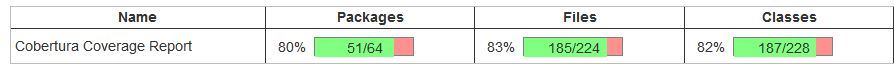
\includegraphics[width=1.0\textwidth]{resources/cobertura-report-new-1}
 	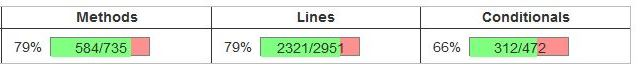
\includegraphics[width=0.7\textwidth]{resources/cobertura-report-new-2}
	\caption[Pokrytí testy po provedených vylepšení]{Pokrytí testy vytvořeného řešení týmového projektu}\label{fig:cober-new}
\end{figure}


\begin{conclusion}
	%sem napište závěr Vaší práce
\end{conclusion}

\bibliographystyle{csn690}

\bibliography{mybibliografy}

\appendix
\chapter{Seznam použitých zkratek}
% \printglossaries
\begin{description}
	\item[EAN] European Article Number
	\item[XML] Extensible markup language
	\item[HTML] Hypertext Markup Language
	\item[CSS] Cascading style sheets
	\item[JSON] JavaScript Object Notation
	\item[HTTP] Hypertext Transfer Protocol
	\item[DAO] Data Access Object
	\item[URL] Uniform Resource Locator

\end{description}


% % % % % % % % % % % % % % % % % % % % % % % % % % % % 
% % Tuto kapitolu z výsledné práce ODSTRAŇTE.
% % % % % % % % % % % % % % % % % % % % % % % % % % % % 
% 
% \chapter{Návod k~použití této šablony}
% 
% Tento dokument slouží jako základ pro napsání závěrečné práce na Fakultě informačních technologií ČVUT v~Praze.
% 
% \section{Výběr základu}
% 
% Vyberte si šablonu podle druhu práce (bakalářská, diplomová), jazyka (čeština, angličtina) a kódování (ASCII, \mbox{UTF-8}, \mbox{ISO-8859-2} neboli latin2 a nebo \mbox{Windows-1250}). 
% 
% V~české variantě naleznete šablony v~souborech pojmenovaných ve formátu práce\_kódování.tex. Typ může být:
% \begin{description}
% 	\item[BP] bakalářská práce,
% 	\item[DP] diplomová (magisterská) práce.
% \end{description}
% Kódování, ve kterém chcete psát, může být:
% \begin{description}
% 	\item[UTF-8] kódování Unicode,
% 	\item[ISO-8859-2] latin2,
% 	\item[Windows-1250] znaková sada 1250 Windows.
% \end{description}
% V~případě nejistoty ohledně kódování doporučujeme následující postup:
% \begin{enumerate}
% 	\item Otevřete šablony pro kódování UTF-8 v~editoru prostého textu, který chcete pro psaní práce použít -- pokud můžete texty s~diakritikou normálně přečíst, použijte tuto šablonu.
% 	\item V~opačném případě postupujte dále podle toho, jaký operační systém používáte:
% 	\begin{itemize}
% 		\item v~případě Windows použijte šablonu pro kódování \mbox{Windows-1250},
% 		\item jinak zkuste použít šablonu pro kódování \mbox{ISO-8859-2}.
% 	\end{itemize}
% \end{enumerate}
% 
% 
% V~anglické variantě jsou šablony pojmenované podle typu práce, možnosti jsou:
% \begin{description}
% 	\item[bachelors] bakalářská práce,
% 	\item[masters] diplomová (magisterská) práce.
% \end{description}
% 
% \section{Použití šablony}
% 
% Šablona je určena pro zpracování systémem \LaTeXe{}. Text je možné psát v~textovém editoru jako prostý text, lze však také využít specializovaný editor pro \LaTeX{}, např. Kile.
% 
% Pro získání tisknutelného výstupu z~takto vytvořeného souboru použijte příkaz \verb|pdflatex|, kterému předáte cestu k~souboru jako parametr. Vhodný editor pro \LaTeX{} toto udělá za Vás. \verb|pdfcslatex| ani \verb|cslatex| \emph{nebudou} s~těmito šablonami fungovat.
% 
% Více informací o~použití systému \LaTeX{} najdete např. v~\cite{wikilatex}.
% 
% \subsection{Typografie}
% 
% Při psaní dodržujte typografické konvence zvoleného jazyka. České \uv{uvozovky} zapisujte použitím příkazu \verb|\uv|, kterému v~parametru předáte text, jenž má být v~uvozovkách. Anglické otevírací uvozovky se v~\LaTeX{}u zadávají jako dva zpětné apostrofy, uzavírací uvozovky jako dva apostrofy. Často chybně uváděný symbol "{} (palce) nemá s~uvozovkami nic společného.
% 
% Dále je třeba zabránit zalomení řádky mezi některými slovy, v~češtině např. za jednopísmennými předložkami a spojkami (vyjma \uv{a}). To docílíte vložením pružné nezalomitelné mezery -- znakem \texttt{\textasciitilde}. V~tomto případě to není třeba dělat ručně, lze použít program \verb|vlna|.
% 
% Více o~typografii viz \cite{kobltypo}.
% 
% \subsection{Obrázky}
% 
% Pro umožnění vkládání obrázků je vhodné použít balíček \verb|graphicx|, samotné vložení se provede příkazem \verb|\includegraphics|. Takto je možné vkládat obrázky ve formátu PDF, PNG a JPEG jestliže používáte pdf\LaTeX{} nebo ve formátu EPS jestliže používáte \LaTeX{}. Doporučujeme preferovat vektorové obrázky před rastrovými (vyjma fotografií).
% 
% \subsubsection{Získání vhodného formátu}
% 
% Pro získání vektorových formátů PDF nebo EPS z~jiných lze použít některý z~vektorových grafických editorů. Pro převod rastrového obrázku na vektorový lze použít rasterizaci, kterou mnohé editory zvládají (např. Inkscape). Pro konverze lze použít též nástroje pro dávkové zpracování běžně dodávané s~\LaTeX{}em, např. \verb|epstopdf|.
% 
% \subsubsection{Plovoucí prostředí}
% 
% Příkazem \verb|\includegraphics| lze obrázky vkládat přímo, doporučujeme však použít plovoucí prostředí, konkrétně \verb|figure|. Například obrázek \ref{fig:float} byl vložen tímto způsobem. Vůbec přitom nevadí, když je obrázek umístěn jinde, než bylo původně zamýšleno -- je tomu tak hlavně kvůli dodržení typografických konvencí. Namísto vynucování konkrétní pozice obrázku doporučujeme používat odkazování z~textu (dvojice příkazů \verb|\label| a \verb|\ref|).
% 
% \begin{figure}\centering
% 	
\includegraphics[width=0.5\textwidth, angle=30]{cvut-logo-bw}
% 	\caption[Příklad obrázku]{Ukázkový obrázek v~plovoucím prostředí}\label{fig:float}
% \end{figure}
% 
% \subsubsection{Verze obrázků}
% 
% % Gnuplot BW i barevně
% Může se hodit mít více verzí stejného obrázku, např. pro barevný či černobílý tisk a nebo pro prezentaci. S~pomocí některých nástrojů na generování grafiky je to snadné.
% 
% Máte-li například graf vytvořený v programu Gnuplot, můžete jeho černobílou variantu (viz obr. \ref{fig:gnuplot-bw}) vytvořit parametrem \verb|monochrome dashed| příkazu \verb|set term|. Barevnou variantu (viz obr. \ref{fig:gnuplot-col}) vhodnou na prezentace lze vytvořit parametrem \verb|colour solid|.
% 
% \begin{figure}\centering
% 	\includegraphics{gnuplot-bw}
% 	\caption{Černobílá varianta obrázku generovaného programem Gnuplot}\label{fig:gnuplot-bw}
% \end{figure}
% 
% \begin{figure}\centering
% 	\includegraphics{gnuplot-col}
% 	\caption{Barevná varianta obrázku generovaného programem Gnuplot}\label{fig:gnuplot-col}
% \end{figure}
% 
% 
% \subsection{Tabulky}
% 
% Tabulky lze zadávat různě, např. v~prostředí \verb|tabular|, avšak pro jejich vkládání platí to samé, co pro obrázky -- použijte plovoucí prostředí, v~tomto případě \verb|table|. Například tabulka \ref{tab:matematika} byla vložena tímto způsobem.
% 
% \begin{table}\centering
% 	\caption[Příklad tabulky]{Zadávání matematiky}\label{tab:matematika}
% 	\begin{tabular}{|l|l|c|c|}\hline
% 		Typ		& Prostředí		& \LaTeX{}ovská zkratka	& \TeX{}ovská zkratka	\tabularnewline \hline \hline
% 		Text		& \verb|math|		& \verb|\(...\)|	& \verb|$...$|		\tabularnewline \hline
% 		Displayed	& \verb|displaymath|	& \verb|\[...\]|	& \verb|$$...$$|	\tabularnewline \hline
% 	\end{tabular}
% \end{table}
% 
% % % % % % % % % % % % % % % % % % % % % % % % % % % % 

\chapter{Obsah přiloženého CD}

%upravte podle skutecnosti

\begin{figure}
	\dirtree{%
		.1 readme.txt\DTcomment{stručný popis obsahu CD}.
		.1 exe\DTcomment{adresář se spustitelnou formou implementace}.
		.1 src.
		.2 impl\DTcomment{zdrojové kódy implementace}.
		.2 thesis\DTcomment{zdrojová forma práce ve formátu \LaTeX{}}.
		.1 text\DTcomment{text práce}.
		.2 thesis.pdf\DTcomment{text práce ve formátu PDF}.
		.2 thesis.ps\DTcomment{text práce ve formátu PS}.
	}
\end{figure}

\end{document}
